\section{Results and Discussion}

\subsection{Training Dynamics}\label{ssec:training}
Figure~\ref{fig:training} summarizes the 150-episode run. Episode outcomes are dominated
by the demand realization, not by smooth policy improvement: fleet travel time swings from
254.3\,s (episode~59) to 1174.8\,s (episode~63) and correlates strongly with teleports
($r{=}0.81$): the seeds that draw heavy demand gridlock regardless of routing
(panels~a,b). Completion stays high (mean 0.996). Underneath the noise the policy sharpens:
entropy anneals from 0.98 to 0.62 (panel~c) and the mean margin between candidate scores
grows from near zero to 0.89. The policy detours throughout training (per-episode
non-shortest rate 30--60\%), so the routing signal is present in the weights the whole
time. However, the PPO update magnitude stays
small (the approximate KL divergence has a median of only 0.0019 against a 0.015 target and
never trips early stopping, panel~d), so the per-update signal is weak: with many near-equal
parallel routes on a grid, the advantage of any single choice is small and easily buried by
traffic variance. Value-target normalization keeps the critic well-conditioned (median
value loss 0.51). Because later episodes are not reliably faster and the fleet detour
\emph{rate} drifts slowly upward (Section~\ref{ssec:limits}), we select the checkpoint by
held-out greedy evaluation rather than final weights: this picked episode~74, which on the
30-seed selection block (6000--6029) completes every vehicle and runs 27.0\% below Dijkstra
(440.2\,s vs.\ 603.5\,s, 22/30 wins, p90 $-24.2\%$) at a 38.6\% non-shortest rate---the
recalibrated guard now executes rather than reverts the learned detours. That block draws
several catastrophic-congestion seeds the policy roughly halves (e.g.\ seed~6018
$1542\to685$\,s), so its gains run larger than on the disjoint deployment block next.

\begin{figure*}[!t]
\centering
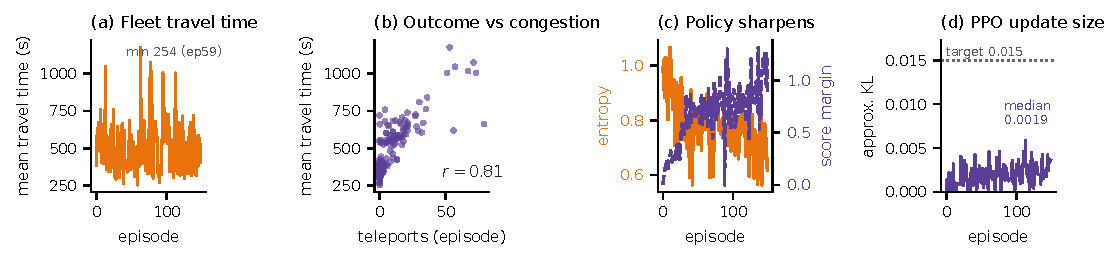
\includegraphics[width=0.92\textwidth]{Images/training_dynamics.pdf}
\caption{MAPPO training over 150 episodes on the congested corridor. (a) Fleet travel time
is highly variable and (b) tracks congestion spikes (teleports): episode outcomes are
demand-driven. (c) Policy entropy anneals and the candidate-score margin grows as the
policy sharpens, but (d) PPO updates stay well below the target KL, indicating a weak
per-update learning signal on a dense grid with many near-equal routes.}
\label{fig:training}
\end{figure*}

\subsection{Deployment: MAPPO vs.\ Dijkstra}
We deploy the selected checkpoint on a \emph{disjoint} block of 20 held-out scenarios
(seeds 4010--4029, never used for training or checkpoint selection) against Dijkstra on
identical demand (Table~\ref{tab:deploy}, Fig.~\ref{fig:deploy}). Both complete 100\% of
vehicles. Greedy MAPPO (with the detour guard active, our default deployment) reduces mean
fleet travel time from 596.6\,s to 534.3\,s ($-10.4\%$, median per-scenario $-33.0$\,s),
winning 15 of 20 scenarios (paired Wilcoxon $p{=}0.019$), and improves p90 travel time
(972\,s vs 1098\,s, $-11.4\%$), the p95/p50 spread (2.07 vs 2.17), and deadline misses (209
vs 225). Here the policy executes a non-shortest route 37.6\% of the time, combining live
replanning with genuine load-spreading detours. The improvement grows with
congestion ($r{=}-0.57$ between per-scenario gain and Dijkstra travel time,
Fig.~\ref{fig:deploy}a): the largest wins are the most congested scenarios (seed~4028
$1109\to702$\,s, seed~4010 $1585\to1282$\,s), while the few losses are light-traffic
scenarios where the shortest path is already near-optimal (seeds 4020, 4014 at $+18$--$38$
\,s). One scenario, seed~4012, is a genuine failure: MAPPO nearly doubles travel time
($664\to1031$\,s), a rare gridlock we return to in Section~\ref{ssec:limits}.

\begin{table}[!t]
\caption{Deployment over 20 Held-Out Scenarios (Seeds 4010--4029)}
\label{tab:deploy}
\centering
\footnotesize
\setlength{\tabcolsep}{3.4pt}
\begin{tabular}{lrrr}
\toprule
Metric & Dijkstra & \shortstack[r]{MAPPO\\(guard on)} & \shortstack[r]{MAPPO\\(guard off)} \\
\midrule
Completion rate       & 1.000 & 1.000 & 1.000 \\
Avg.\ travel time (s) & 596.6 & 534.3 & \textbf{516.9} \\
\quad vs.\ Dijkstra   & --    & $-10.4\%$ & $\mathbf{-13.4\%}$ \\
p50 travel time (s)   & 576.7 & 532.8 & \textbf{504.9} \\
p90 travel time (s)   & 1097.6 & 972.2 & \textbf{939.1} \\
p95/p50 ratio         & 2.17  & \textbf{2.07}  & 2.12 \\
Deadline misses       & 225.4 & 208.8 & \textbf{206.6} \\
Non-shortest rate     & --    & 0.38  & 0.40 \\
Scenarios won         & --    & 15/20 & 15/20 \\
Wilcoxon $p$ vs.\ Dij.\ & --  & 0.019 & \textbf{0.008} \\
\bottomrule
\end{tabular}
\end{table}

\begin{figure*}[!t]
\centering
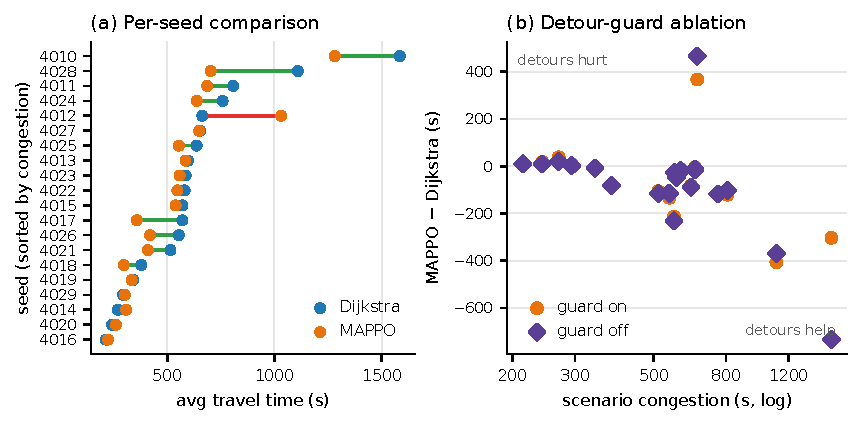
\includegraphics[width=0.78\textwidth]{Images/deployment.pdf}
\caption{Deployment on 20 disjoint held-out scenarios. (a)~Per-scenario fleet travel time,
Dijkstra vs.\ greedy MAPPO (detour guard on), sorted by congestion; green connectors mark
MAPPO wins, red losses, and the largest wins fall on the most congested scenarios
($r{=}-0.57$ between gain and congestion). (b)~Detour-guard ablation: per-scenario gain over
Dijkstra vs.\ scenario congestion (log axis) for the deployed guard-on policy (orange, 38\%
detours) and the guard-off policy (violet, 40\% detours). Removing the guard helps most on
the most congested scenarios (guard-off points fall below guard-on on the right, e.g.\ the
rightmost pair) and is roughly neutral in light traffic; the lone point far above zero is the
seed~4012 gridlock, where both configurations fail.}
\label{fig:deploy}
\end{figure*}

\subsection{When Do Selfless Detours Help? A Detour-Guard Ablation}\label{ssec:ablation}
The deployed policy already executes 37.6\% non-shortest routes, so the recalibrated guard
is no longer an on/off switch on selflessness: it reverts only the \emph{pile-on} subset
(detours onto an alternative that is itself near capacity and buys no measurable relief).
Turning it off raises the non-shortest rate only slightly, to 39.9\% (Table~\ref{tab:deploy}),
and lowers mean fleet travel time a further 3\%, to 516.9\,s ($-13.4\%$, Wilcoxon
$p{=}0.008$), with a better p90 (939.1\,s); both configurations win 15/20 and complete every
vehicle.

Where that extra 3\% comes from is the paper's central result: it is concentrated almost
entirely at high congestion (Fig.~\ref{fig:deploy}b). Splitting the 20 scenarios at their
median congestion, removing the guard helps the congested half by $-31$\,s on average but
the light half by only $-4$\,s. The clearest case is the most congested scenario, seed~4010:
guard-on already cuts it $1585\to1282$\,s, and executing the pile-on detours the guard would
revert cuts it much further, to $851$\,s---while in light traffic the two configurations sit
within noise. The guard earns its keep only on the seed~4012 gridlock, where the extra
detours make things slightly worse ($1031\to1130$\,s): a small robustness margin rather
than a large peak-versus-robustness trade.

The value of selfless routing is therefore not a fixed property of the policy; it tracks
the network's price of anarchy: where contention is high the learned detours move vehicles
onto genuine spare capacity and cut fleet travel time, while on a lightly loaded grid
selfish shortest-path routing already approximates the system optimum and every detour is
wasted distance. The recalibrated guard suppresses exactly the detours that relieve nothing.

\subsection{Effect of Controlled-Vehicle Penetration}\label{ssec:penetration}
Figure~\ref{fig:penetration} reports the fixed-demand penetration sweep; completion
stays at 100\% at every level. The typical benefit of the deployed policy grows
monotonically with the controlled share: the median per-scenario gain over Dijkstra
improves from $-4.1$\,s at 10\% penetration to $-18.1$\,s at 25\%, $-20.2$\,s at 50\%,
and $-33$\,s at 75--100\%, with the win rate rising from 11/20 to 15--16/20. The
improvement becomes statistically reliable once the policy controls at least a quarter of
the route-choosing traffic (paired Wilcoxon $p{\le}0.02$ at 25\% and 75--100\%):
coordination needs mass before it can reliably move fleet-level outcomes. Two second-order
effects qualify the trend. First, the policy \emph{chooses} detours more often the less it
controls (non-shortest rate 38\% at full penetration rising to 48\% at 10\%,
Fig.~\ref{fig:penetration}b), consistent with its observations containing more congestion
that no teammate will clear. Second, mean (as opposed to median) gains are erratic at
intermediate penetration, where mixed live/fixed traffic---never seen during training---
produces gridlock outliers (the seed~4012 mode of Section~\ref{ssec:limits}); robust
partial adoption therefore calls for training under mixed autonomy, not just deploying
into it.

\begin{figure}[!t]
\centering
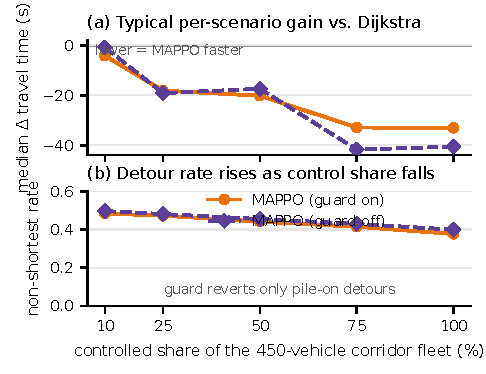
\includegraphics[width=0.94\columnwidth]{Images/penetration_sweep.pdf}
\caption{Fixed-demand penetration sweep on the 20 held-out scenarios. (a)~Median
per-scenario fleet travel-time change vs.\ Dijkstra: the typical gain grows
monotonically with penetration. (b)~With the guard removed, the policy executes
non-shortest routes more often the smaller its share of the fleet.}
\label{fig:penetration}
\end{figure}

\subsection{Greedy vs.\ Stochastic Deployment}\label{ssec:greedy}
Because the recalibrated guard now lets most detours through, greedy (argmax) and
stochastic (sampled) deployment no longer coincide. On the 30 selection seeds (three samples
each, guard active), sampling spreads slightly more load (42\% vs.\ 39\% non-shortest) but
is net slower---477.5\,s vs.\ the greedy 440.2\,s, a paired advantage for greedy on nearly
every seed (sign test $p{=}0.001$)---both completing every vehicle. The argmax already
captures the useful detours while extra sampling mostly adds pile-on choices, so we deploy
greedily; route diversity comes from the policy and the reservation field, not sampling
noise.

\subsection{Limitations}\label{ssec:limits}
Four limitations qualify these results. First, the aggregate gains are driven by a minority
of severe-congestion scenarios; this is arguably the point of selfless routing, but it
inflates means and is why the more-congested selection block ($-27\%$) improves far more
than the disjoint deployment block ($-10.4\%$). Second, one scenario (seed~4012) is a true
failure in which the greedy policy gridlocks and even the guard's pile-on veto does not
prevent it: the coordination guardrails are necessary but not sufficient. Third, because
the reward settles each agent's detour credit on decision-time estimates, the fleet detour
\emph{rate} drifts slowly upward (bounded near 44\%, not divergent), which we currently
contain by best-checkpoint early stopping rather than by a stable attractor---a detour-rate
penalty or counterfactual critic could supply one. Fourth, the weak per-update learning
signal (Section~\ref{ssec:training}) means the policy is likely under-trained, and the
moderate price of anarchy of a dense grid still caps how much any routing policy can gain,
motivating higher-price-of-anarchy networks. The honest contribution is the \emph{conditions}
under which selfless routing helps, not a single benchmark number.
